\documentclass[11pt]{article}

% ---------- Layout ----------
\usepackage[a4paper,margin=1in]{geometry}
\usepackage[T1]{fontenc}
\usepackage{newtxtext,newtxmath}
\usepackage{microtype}
\usepackage{booktabs}
\usepackage{tabularx}
\usepackage{array}
\usepackage{xcolor}
\usepackage[colorlinks=true,linkcolor=teal,citecolor=teal,urlcolor=teal]{hyperref}
\usepackage{titlesec}
\usepackage{fancyhdr}
\usepackage{tikz}
\usetikzlibrary{arrows.meta,positioning,fit,backgrounds}
\usepackage{caption}
\usepackage{enumitem}
\usepackage{amsmath}
\usepackage{graphicx}
\usepackage{pgfplots}
\pgfplotsset{compat=1.18}
\usepgfplotslibrary{fillbetween}

\definecolor{ink}{HTML}{1B2A2A}
\definecolor{teal}{HTML}{1F6F6B}
\definecolor{sand}{HTML}{F3EFE6}
\definecolor{rust}{HTML}{A34A28}

\captionsetup{font=small,labelfont={bf,color=teal},skip=6pt}
\titleformat{\section}{\normalfont\large\bfseries\color{teal}}{\thesection}{0.6em}{}
\titleformat{\subsection}{\normalfont\normalsize\bfseries\color{ink}}{\thesubsection}{0.5em}{}
\titlespacing*{\section}{0pt}{14pt}{6pt}
\titlespacing*{\subsection}{0pt}{10pt}{4pt}

\pagestyle{fancy}
\fancyhf{}
\renewcommand{\headrulewidth}{0.4pt}
\fancyhead[L]{\footnotesize\color{ink}Three Modalities, Three Tracks}
\fancyhead[R]{\footnotesize\color{ink}CS 668 · Pace University}
\fancyfoot[C]{\footnotesize\thepage}

\setlength{\parskip}{2pt}
\setlength{\parindent}{0pt}
\setlength{\emergencystretch}{2em}
\newcommand{\best}[1]{\textbf{#1}}

\title{\vspace{-1.2em}\bfseries\LARGE Three Modalities, Three Tracks\\[2pt]
\large Text, Image, and Combined Baselines for Multimodal Misinformation Detection}
\author{
  Rafiul Haider\thanks{Combined track; corresponding author.} \quad
  Harika Etikela\thanks{Text track.} \quad
  Ananya\thanks{Image track.} % TODO: add full surname before submission
  \\[4pt]
  \small CS 668 Analytics Capstone · Pace University · Instructor: Dr. Krishna Bathula
}
\date{October 2026}

\begin{document}
\maketitle

\begin{abstract}
Misinformation is not one task. A claim can be false in its text, an image can be generated, and a real image and a real caption can be paired out of context. We report three coordinated experiments that measure each channel and then a combined detector. On \textbf{WELFake}, a cleaned 63{,}678-article corpus with a stratified 70/15/15 split, classical TF--IDF models reach 87.6--97.4\% test accuracy and a short DistilBERT run reaches 98.3\%; source and style cues explain much of the signal. On \textbf{CIFAKE}, a cleaned 3{,}986-image test split, a fine-tuned ResNet-18 reaches 96.3\% accuracy and AUC 0.995, but mild blur lowers accuracy to 85.6\%, showing reliance on fine detail. On the \textbf{combined} track, a frozen LAYA-Vision checkpoint is evaluated zero-shot on MMFakeBench, VERITE, and NewsCLIPpings. It reaches 20.37\% four-class macro-F1 on the MMFakeBench official test, 35.66\% three-class accuracy on VERITE, and 50.83\% on NewsCLIPpings. The matched text-only control scores 21.81\% macro-F1, so the image adds nothing measurable; a source-name rule reaches 91.5\% on the same test rows. A frozen-feature linear probe improves held-out NewsCLIPpings test accuracy from 51.1\% to 57.4\%, identifying headroom for fine-tuning. We report these as post-hoc, single-checkpoint baselines and specify the fine-tuning programme, compute setup, and six-condition evaluation that follow.
\end{abstract}

\begin{figure}[t]
\centering
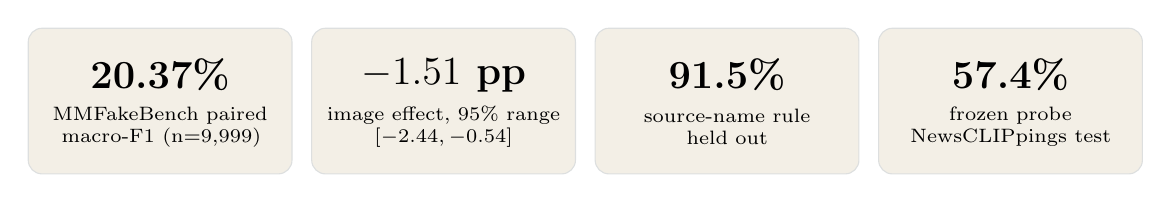
\begin{tikzpicture}
\newcommand{\statcard}[3]{%
  \begin{scope}[shift={(#1,0)}]
    \node[draw=ink!15,rounded corners=5pt,fill=sand,minimum width=3.35cm,minimum height=1.85cm] (bg) {};
    \node[font=\Large\bfseries] at (0,0.33) {#2};
    \node[font=\scriptsize,align=center,text width=3.05cm] at (0,-0.33) {#3};
  \end{scope}}
\statcard{0}{20.37\%}{MMFakeBench paired\\macro-F1 (n=9{,}999)}
\statcard{3.6}{$-1.51$ pp}{image effect, 95\% range\\$[-2.44,-0.54]$}
\statcard{7.2}{91.5\%}{source-name rule\\held out}
\statcard{10.8}{57.4\%}{frozen probe\\NewsCLIPpings test}
\end{tikzpicture}
\caption{Four numbers that frame the paper: the paired baseline, the image effect, the benchmark shortcut, and the headroom a trained head recovers. Each is a different task; they are not a ranking.}
\label{fig:glance}
\end{figure}


\section{Introduction}

A multimodal misinformation detector is usually described as one model, but it answers at least three different questions. Is the \emph{text} false? Is the \emph{image} synthetic or manipulated? Is a genuine image paired with a genuine caption that belongs to a different event? Each question has its own benchmark, its own label contract, and its own shortcuts. Treating them as one accuracy number hides the differences that matter.

This paper reports three coordinated experiments. The \emph{text track} asks whether article text alone separates real from fake news on WELFake \cite{welfake}. The \emph{image track} asks whether a detector separates real from AI-generated images on CIFAKE \cite{cifake}, and whether that detector survives simple perturbations. The \emph{combined track} evaluates a frozen vision-language checkpoint, LAYA-Vision \cite{laya}, on three misinformation benchmarks: MMFakeBench \cite{mmfakebench}, VERITE \cite{verite}, and NewsCLIPpings \cite{newsclippings}. It then adds a frozen-feature probe to estimate the headroom that fine-tuning could exploit.

Our contributions are:
\begin{enumerate}[leftmargin=1.4em,itemsep=2pt]
  \item A reproducible text baseline on WELFake with explicit source-cue diagnostics and a documented transformer-budget caveat.
  \item A cleaned CIFAKE image baseline with duplicate/leakage removal, a five-rung model ladder, and perturbation stress tests that expose reliance on fine detail.
  \item A verified zero-shot combined baseline with matched modality controls, cluster-aware ranges, calibration, a source-metadata audit, and a frozen-feature transfer probe.
  \item A concrete, pre-registered fine-tuning plan: six comparison conditions, two fusion heads over frozen LAYA features, three seeds, held-out targets, and an explicit compute and ethics setup.
\end{enumerate}

The headline is deliberately negative. On the combined track the image did not help, and MMFakeBench is largely solvable from source names. That is a benchmark finding, not a model failure, and it changes what the fine-tuning stage should measure.

\section{Related Work}

\textbf{Text.} WELFake \cite{welfake} introduced word-embedding and linguistic features for fake-news detection and is a standard public corpus. Classical TF--IDF pipelines remain strong baselines, and DistilBERT \cite{distilbert} offers a compact transformer alternative. A recurring confound is that source and format cues (for example, the token ``reuters'') correlate with the label.

\textbf{Images.} CNN detectors trained on one generator can transfer poorly to another \cite{wang2020}, while frequency and diffusion-specific artifacts provide complementary signal \cite{frank2020,corvi2023}. CIFAKE \cite{cifake} provides a balanced 120{,}000-image benchmark of CIFAR-10 reals and Stable Diffusion fakes. GenImage \cite{genimage} and universal-detector work \cite{ojha2023} make cross-generator evaluation the central question; AEROBLADE \cite{aeroblade} and CLIP-based detectors \cite{cozzolino2024} explore training-free and few-shot routes respectively.

\textbf{Combined.} MMFakeBench \cite{mmfakebench} labels original items, textual distortion, visual distortion, and mismatch. VERITE \cite{verite} labels true, miscaptioned, and out-of-context pairs, with modality balancing. NewsCLIPpings \cite{newsclippings} labels pristine versus falsified image--caption pairs. LAMAR \cite{lamar} reports strong end-to-end results on these tasks; its binary true-versus-out-of-context targets (84.8\% NewsCLIPpings, 76.3\% VERITE) are the reference points our fine-tuning plan adopts. Our zero-shot baseline is not comparable to those trained systems, and we do not present it as such.

\section{Datasets}

\begin{table}[t]
\centering
\small
\caption{Datasets and evaluation populations. Native tasks and metrics are kept separate; numbers are not pooled across rows.}
\label{tab:data}
\begin{tabularx}{\textwidth}{@{}l l r r X@{}}
\toprule
\textbf{Track} & \textbf{Dataset} & \textbf{Rows used} & \textbf{Classes} & \textbf{Protocol notes} \\
\midrule
Text & WELFake & 63{,}678 & 2 & 8{,}456 exact duplicates removed; stratified 70/15/15 (44{,}574 / 9{,}552 / 9{,}552). \\
Image & CIFAKE & 10{,}000 / 1{,}996 / 3{,}986 & 2 & Cleaned subset (train/val/test); 32$\times$32; FAKE positive; test scored once. \\
Combined & MMFakeBench & 9{,}999 / 10{,}000 & 4 & Official test, post-hoc; one image decode error retained in attempted coverage. \\
Combined & VERITE & 1{,}001 & 3 & Current repository CSV; README describes 1{,}000; all rows kept. \\
Combined & NewsCLIPpings & 7{,}024 & 2 & Validation annotations; images streamed, not stored; terms unresolved. \\
\bottomrule
\end{tabularx}
\end{table}

Table~\ref{tab:data} summarises the populations. Three properties are worth stating up front.

\textbf{Leakage and overlap.} The MMFakeBench Stage~00 audit found 28 image-byte duplicate groups crossing the validation/test boundary, 53 duplicate normalized-text groups covering 109 test rows, and three normalized text strings shared with validation. Nine exposed validation rows share exact image bytes with test records through 14 hash edges. The CIFAKE audit found 2{,}218 duplicate files in train, 454 in test, and 378 shared files; after removing pixel-identical images the clean test split has zero shared with train. The text track removes exact duplicates before splitting.

\textbf{Exposure.} The MMFakeBench official test split was inspected in earlier work, so every test number in this paper is a post-hoc diagnostic, not blind confirmation. The NewsCLIPpings test split was read once, after the transfer-probe protocol was frozen, and is treated as held out for that probe.

\textbf{Source metadata.} MMFakeBench rows carry \texttt{text\_source} and \texttt{image\_source}. These are audit variables, not model inputs. We fit a two-column rule on the 1{,}000 validation rows and apply it to test; it reaches 91.5\% accuracy and 85.1\% macro-F1, and 13 of 14 source pairs are label-pure.

\section{Method}

\subsection{Text track}

We remove exact duplicates, freeze a stratified 70/15/15 split, and compare TF--IDF representations with Naive Bayes, logistic regression, linear SVM, and random forest. The linear SVM is run three ways: cleaned text, raw text, and raw text with the token ``reuters'' removed. A DistilBERT model is run on a 5{,}000-article, one-epoch budget as an exploratory check. Models are selected on validation; test is scored once. Preprocessing keeps case and exclamation marks in one variant because the EDA shows they differ by class.

\subsection{Image track}

We use a balanced 10{,}000-image training subset, 1{,}996 validation images, and 3{,}986 test images after duplicate removal. Five rungs are compared: an always-guess floor; 21 handcrafted statistics with logistic regression and with random forest; a small CNN trained from scratch; ResNet-18 \cite{resnet} frozen with a logistic head; and ResNet-18 fine-tuned. FAKE is the positive class. Validation selects the epoch, test is scored once, and 95\% bootstrap intervals use seed~42. Diagnosis includes single-feature AUCs, frequency-family ablations, blur/JPEG/grayscale stress tests, patch shuffling, and Grad-CAM \cite{gradcam}.

\subsection{Combined track}

The checkpoint is LAYA-Vision revision \texttt{f2fe3c12\ldots}, a 201M-parameter SmolVLM-based model \cite{smolvlm}, run on CPU in fp32 with one fixed question bank. Three arms are defined by what the model receives: image + text (paired), text only, and image only. The text-only arm is a matched control on the same rows; the image-only arm uses a 1{,}000-row seeded, unstratified sample. Questions, options, and decoding are fixed; no prompt or threshold selection is performed on test.

\begin{figure}[t]
\centering
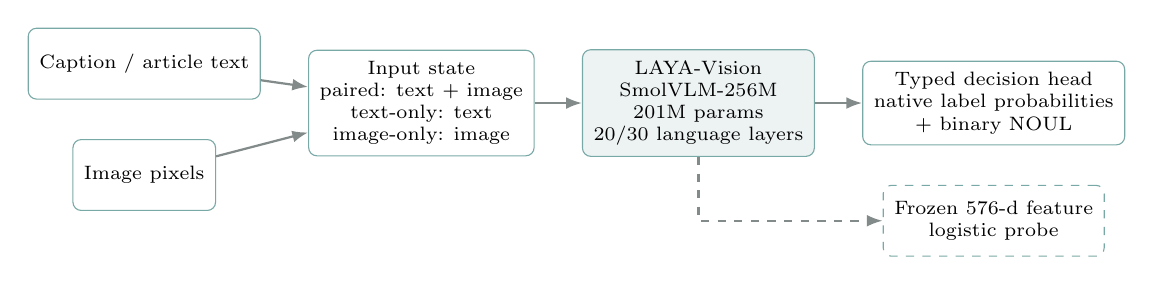
\begin{tikzpicture}[
  node distance=5mm and 6mm,
  box/.style={draw=teal!60,rounded corners=3pt,fill=white,align=center,inner sep=4pt,font=\scriptsize,minimum height=9mm},
  arr/.style={-{Latex[length=2mm]},draw=ink!55,thick}
]
\node[box] (text) {Caption / article text};
\node[box,below=of text] (image) {Image pixels};
\node[box,right=of text,yshift=-5mm] (state) {Input state\\paired: text + image\\text-only: text\\image-only: image};
\node[box,right=of state,fill=teal!8] (model) {LAYA-Vision\\SmolVLM-256M\\201M params\\20/30 language layers};
\node[box,right=of model] (head) {Typed decision head\\native label probabilities\\+ binary NOUL};
\node[box,below=of head,dashed] (probe) {Frozen 576-d feature\\logistic probe};
\draw[arr] (text) -- (state);
\draw[arr] (image) -- (state);
\draw[arr] (state) -- (model);
\draw[arr] (model) -- (head);
\draw[arr,dashed] (model.south) |- (probe.west);
\end{tikzpicture}
\caption{How LAYA-Vision is used. The checkpoint is frozen. Three arms differ only in the input state; the probe reads the 576-dimensional decision feature and never updates the model.}
\label{fig:laya}
\end{figure}


Accuracy, macro-F1, per-class precision/recall/F1, and confusion matrices are computed from saved predictions. Calibration is reported as expected calibration error (ECE, 15 equal-width bins except NewsCLIPpings, where the saved metric uses 10) and Brier score. Uncertainty is a percentile bootstrap over exact image-byte clusters (2{,}000 resamples, seed 20261018), reported as a descriptive range. Paired differences are computed on shared rows only.

\begin{table}[t]
\centering
\small
\caption{The LAYA-Vision setup in detail. Everything here is fixed before evaluation.}
\label{tab:laya}
\begin{tabularx}{\textwidth}{@{}l X@{}}
\toprule
\textbf{Item} & \textbf{Value} \\
\midrule
Checkpoint & LAYA-Vision, revision \texttt{f2fe3c12\ldots} \\
Base model & SmolVLM-256M-Instruct; 201M parameters; 20 of 30 language layers retained \\
Decision feature & 576-dimensional pooled state used by the decision head \\
Arms & Paired \{\texttt{context}, \texttt{image}\}; text-only \{\texttt{context}\}; image-only \{\texttt{image}\} \\
Outputs & Native label probabilities (4, 3, or 2 classes) plus a separate binary NOUL score \\
Runtime & CPU, fp32, batch 4, one fixed question bank, no permutations on test \\
Probe & 71{,}072 train / 7{,}024 validation / 7{,}264 test / 663 VERITE rows; $\lambda$ selected on validation; test read once \\
Verification & 22/22 pipeline gates; 28/28 independent audit; tier-0 max delta 0.0 \\
\bottomrule
\end{tabularx}
\end{table}

\subsection{Frozen-feature probe}
A frozen-feature probe follows the published train-on-NewsCLIPpings, test-on-target protocol. A hook records the 576-dimensional state that LAYA's decision head uses; a logistic regression is fit on 71{,}072 NewsCLIPpings train rows; $\lambda$ is selected on 7{,}024 validation rows; the probe is scored once on the 7{,}264-row NewsCLIPpings test split and on the 663 VERITE true/out-of-context rows. LAYA's weights never change.

\begin{figure}[t]
\centering
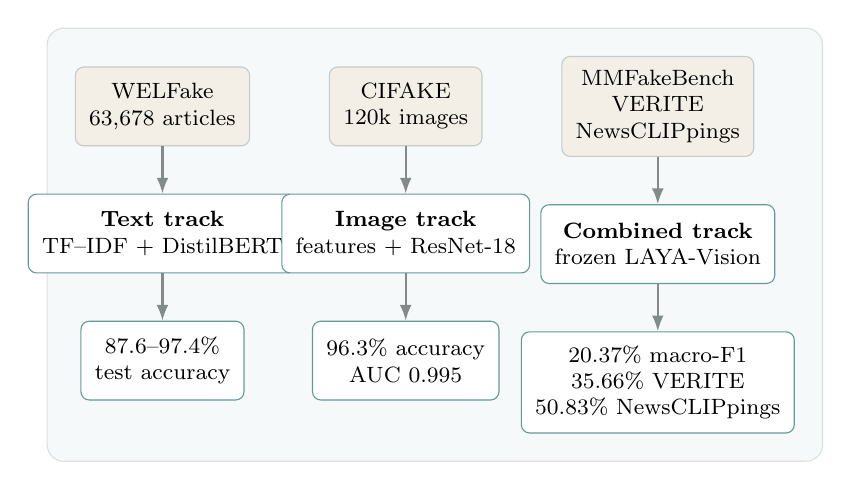
\begin{tikzpicture}[
  node distance=6mm and 10mm,
  box/.style={draw=teal!70,rounded corners=3pt,fill=white,align=center,inner sep=5pt,font=\footnotesize,minimum height=10mm},
  data/.style={draw=ink!25,rounded corners=3pt,fill=sand,align=center,inner sep=5pt,font=\footnotesize,minimum height=10mm},
  arr/.style={-{Latex[length=2mm]},draw=ink!55,thick}
]
\node[data] (w) {WELFake\\63{,}678 articles};
\node[data,right=of w] (c) {CIFAKE\\120k images};
\node[data,right=of c] (m) {MMFakeBench\\VERITE\\NewsCLIPpings};

\node[box,below=of w] (t) {\textbf{Text track}\\TF--IDF + DistilBERT};
\node[box,below=of c] (i) {\textbf{Image track}\\features + ResNet-18};
\node[box,below=of m] (x) {\textbf{Combined track}\\frozen LAYA-Vision};

\draw[arr] (w) -- (t);
\draw[arr] (c) -- (i);
\draw[arr] (m) -- (x);

\node[box,below=of t] (tr) {87.6--97.4\%\\test accuracy};
\node[box,below=of i] (ir) {96.3\% accuracy\\AUC 0.995};
\node[box,below=of x] (xr) {20.37\% macro-F1\\35.66\% VERITE\\50.83\% NewsCLIPpings};

\draw[arr] (t) -- (tr);
\draw[arr] (i) -- (ir);
\draw[arr] (x) -- (xr);

\begin{scope}[on background layer]
  \node[draw=ink!15,rounded corners=6pt,fill=teal!4,fit=(w)(c)(m)(tr)(ir)(xr),inner sep=10pt] {};
\end{scope}
\end{tikzpicture}
\caption{The three-track design. Each track keeps its own dataset, label contract, and metric; the combined track is a zero-shot baseline plus a frozen-feature probe, not a fusion of the text and image models.}
\label{fig:tracks}
\end{figure}

\section{Results}

\subsection{Text track}

\begin{table}[t]
\centering
\small
\caption{WELFake results (accuracy, \%). Validation selects the model; test is scored once. The DistilBERT row used a 5{,}000-article, one-epoch budget and is exploratory.}
\label{tab:text}
\begin{tabular}{@{}lrr@{}}
\toprule
\textbf{Model} & \textbf{Validation} & \textbf{Test} \\
\midrule
Naive Bayes & 87.71 & 87.60 \\
Random Forest & 94.15 & 93.84 \\
Logistic Regression & 95.63 & 95.24 \\
Linear SVM (cleaned text) & 96.79 & 96.49 \\
Linear SVM (raw text) & 97.35 & 97.44 \\
Linear SVM (without ``reuters'') & 96.40 & 96.16 \\
DistilBERT (exploratory) & 98.05 & 98.28 \\
\bottomrule
\end{tabular}
\end{table}


\begin{figure}[t]
\centering
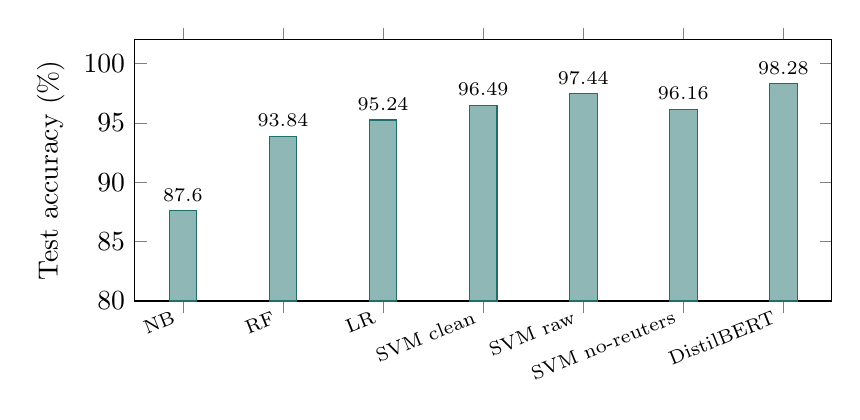
\begin{tikzpicture}
\begin{axis}[
  width=0.86\textwidth,height=4.9cm,ybar,bar width=10pt,ymin=80,ymax=102,clip=false,
  symbolic x coords={NB,RF,LR,SVM clean,SVM raw,SVM no-reuters,DistilBERT},xtick=data,
  x tick label style={rotate=22,anchor=east,font=\scriptsize},
  ylabel={Test accuracy (\%)},enlarge x limits=0.08,
  nodes near coords,nodes near coords style={font=\scriptsize}
]
\addplot[fill=teal!50,draw=teal] coordinates {(NB,87.60) (RF,93.84) (LR,95.24) (SVM clean,96.49) (SVM raw,97.44) (SVM no-reuters,96.16) (DistilBERT,98.28)};
\end{axis}
\end{tikzpicture}
\caption{WELFake test accuracy. The DistilBERT bar used a 5{,}000-article, one-epoch budget; it is exploratory, not a fair transformer comparison. Removing ``reuters'' costs about 1.3 points.}
\label{fig:textbars}
\end{figure}

The floor is 54.6\% (always Real). Removing ``reuters'' costs about 1.3 points on test, evidence that a source cue contributes. The EDA also shows strong style differences: mean capital-letter share 4.93\% versus 7.88\%, exclamation marks in 8\% versus 35\% of articles, and ``video'' in 7.6\% versus 34.4\%. These are dataset properties, not model reasoning; they motivate the source-cue control and the deliberately small transformer claim.

\subsection{Image track}

\begin{table}[t]
\centering
\small
\caption{CIFAKE results on the clean 3{,}986-image test split. FAKE is positive; intervals are 95\% bootstrap ranges.}
\label{tab:image}
\begin{tabular}{@{}lrrr@{}}
\toprule
\textbf{Model} & \textbf{Accuracy [95\% range]} & \textbf{Macro-F1} & \textbf{AUC} \\
\midrule
Always-guess & 49.8 [48.3, 51.4] & 66.5 & 0.500 \\
21 features + logistic & 86.8 [85.6, 87.8] & 86.6 & 0.933 \\
21 features + random forest & 87.9 [86.9, 88.9] & 88.0 & 0.946 \\
Small CNN (scratch) & 94.2 [93.5, 94.9] & 94.1 & 0.986 \\
ResNet-18 frozen + logistic & 88.1 [87.1, 89.0] & 88.1 & 0.948 \\
ResNet-18 fine-tuned & \best{96.3} [95.7, 96.8] & \best{96.2} & \best{0.995} \\
\bottomrule
\end{tabular}
\end{table}


\begin{figure}[t]
\centering
\begin{minipage}{0.49\textwidth}\centering
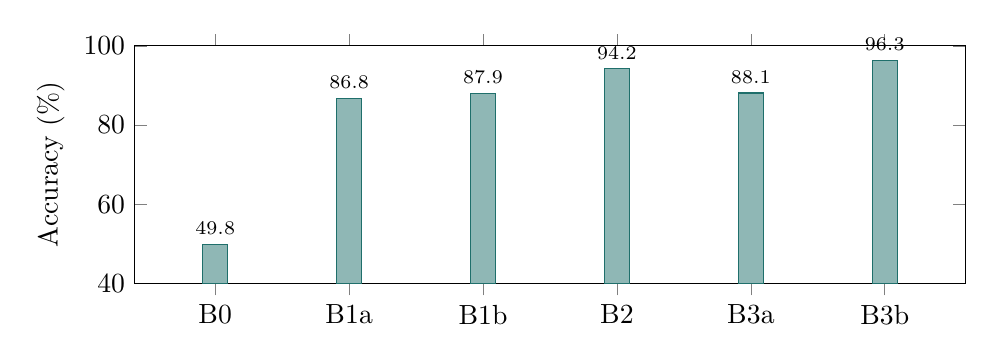
\begin{tikzpicture}
\begin{axis}[width=\textwidth,height=4.6cm,ybar,bar width=9pt,ymin=40,ymax=100,
  symbolic x coords={B0,B1a,B1b,B2,B3a,B3b},xtick=data,
  ylabel={Accuracy (\%)},enlarge x limits=0.12,
  nodes near coords,nodes near coords style={font=\scriptsize}]
\addplot[fill=teal!50,draw=teal] coordinates {(B0,49.8) (B1a,86.8) (B1b,87.9) (B2,94.2) (B3a,88.1) (B3b,96.3)};
\end{axis}
\end{tikzpicture}
\end{minipage}\hfill
\begin{minipage}{0.49\textwidth}\centering
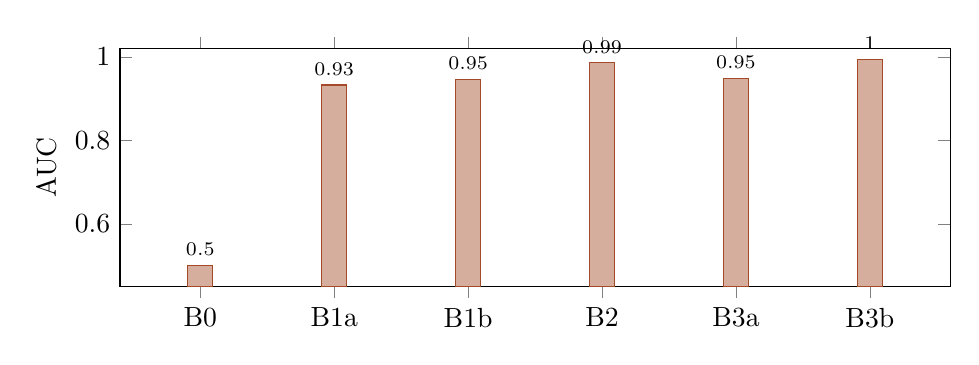
\begin{tikzpicture}
\begin{axis}[width=\textwidth,height=4.6cm,ybar,bar width=9pt,ymin=0.45,ymax=1.02,
  symbolic x coords={B0,B1a,B1b,B2,B3a,B3b},xtick=data,
  ylabel={AUC},enlarge x limits=0.12,
  nodes near coords,nodes near coords style={font=\scriptsize}]
\addplot[fill=rust!45,draw=rust] coordinates {(B0,0.500) (B1a,0.933) (B1b,0.946) (B2,0.986) (B3a,0.948) (B3b,0.995)};
\end{axis}
\end{tikzpicture}
\end{minipage}
\caption{CIFAKE model ladder: B0 floor, B1a/B1b handcrafted features, B2 small CNN, B3a frozen ResNet-18, B3b fine-tuned ResNet-18. Accuracy (left) and AUC (right); FAKE is positive.}
\label{fig:imgbars}
\end{figure}

The best single feature is the finest FFT band (AUC 0.766); 21 features together reach 0.93--0.95, and colour alone only 0.65. Fine detail carries the signal. That is also the fragility: blur $\sigma{=}1$ drops ResNet-18 AUC from 0.995 to 0.77, and mild blur $\sigma{=}0.5$ drops accuracy from 96.3\% to 85.6\%. Grayscale and JPEG quality 75 change little. The model has learned a real but brittle cue.

\subsection{Combined track}

\begin{table}[t]
\centering
\small
\caption{Combined-track results. Native metrics are not comparable across datasets. MMFakeBench and VERITE are post-hoc; the NewsCLIPpings probe test split is held out.}
\label{tab:combined}
\begin{tabularx}{\textwidth}{@{}l l r r r X@{}}
\toprule
\textbf{Dataset} & \textbf{Arm} & \textbf{n} & \textbf{Accuracy} & \textbf{Macro-F1} & \textbf{Note} \\
\midrule
MMFakeBench & Paired & 9{,}999 & 26.42 & 20.37 & 4-class; post-hoc \\
MMFakeBench & Text only & 10{,}000 & 27.93 & 21.81 & matched control \\
MMFakeBench & Image only & 1{,}000 & 26.10 & 19.70 & unstratified sample \\
VERITE & Paired & 1{,}001 & 35.66 & 34.58 & 3-class \\
VERITE & Text only & 1{,}001 & 35.86 & 35.83 & image-independent \\
NewsCLIPpings & Zero-shot & 7{,}024 & 50.83 & 41.85 & chance \\
NewsCLIPpings & Frozen probe & 7{,}264 & \best{57.4} & 57.4 & held-out test \\
VERITE (true/OOC) & Frozen probe & 663 & \best{54.9} & 53.6 & binary transfer \\
\bottomrule
\end{tabularx}
\end{table}


\begin{figure}[t]
\centering
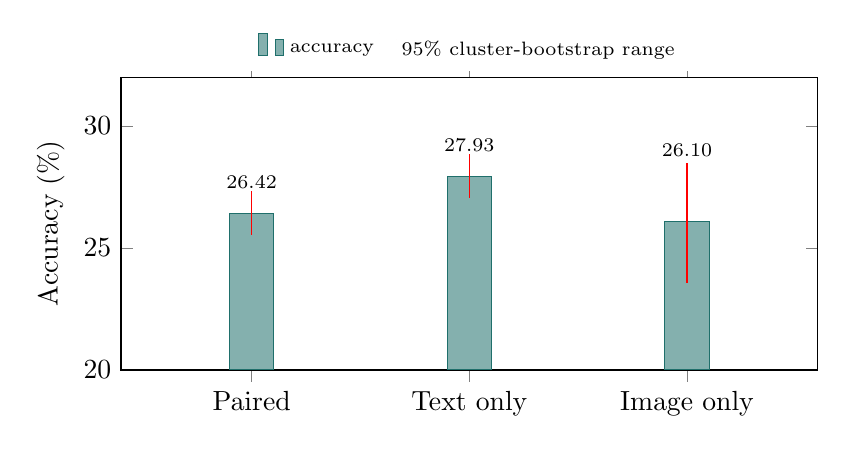
\begin{tikzpicture}
\begin{axis}[
  width=0.86\textwidth,height=5.3cm,
  ybar,bar width=16pt,ymin=20,ymax=32,
  symbolic x coords={Paired,Text only,Image only},xtick=data,
  ylabel={Accuracy (\%)},enlarge x limits=0.30,
  legend style={draw=none,font=\scriptsize,at={(0.5,1.02)},anchor=south,legend columns=2}
]
\addplot[fill=teal!55,draw=teal] coordinates {(Paired,26.42) (Text only,27.93) (Image only,26.10)};
\addlegendentry{accuracy}
\addplot+[only marks,mark=*,mark size=0pt,error bars/.cd,y dir=both,y explicit] coordinates {(Paired,26.42) += (0,0.92) -= (0,0.89) (Text only,27.93) += (0,0.92) -= (0,0.88) (Image only,26.10) += (0,2.37) -= (0,2.52)};
\addlegendentry{95\% cluster-bootstrap range}
\node[font=\scriptsize] at (axis cs:Paired,27.7) {26.42};
\node[font=\scriptsize] at (axis cs:Text only,29.2) {27.93};
\node[font=\scriptsize] at (axis cs:Image only,29.0) {26.10};
\end{axis}
\end{tikzpicture}
\caption{MMFakeBench official test, accuracy with 95\% ranges. The image-only arm is a 1{,}000-row unstratified sample; its range is wider and is not a full-test estimate.}
\label{fig:mmbars}
\end{figure}

Three findings stand out. First, the image does not help: paired minus text-only is $-1.51$ pp on MMFakeBench, 95\% range $[-2.44, -0.54]$, and $-0.20$ pp on VERITE, range $[-3.60, 3.10]$. Second, text-only is better calibrated (ECE 1.23\% versus 8.15\% on MMFakeBench; 4.04\% versus 9.55\% on VERITE). Third, the benchmark is shortcut-solvable: the source-name rule reaches 91.5\%, and its in-sample ceiling is 95.0\%.


\begin{figure}[t]
\centering
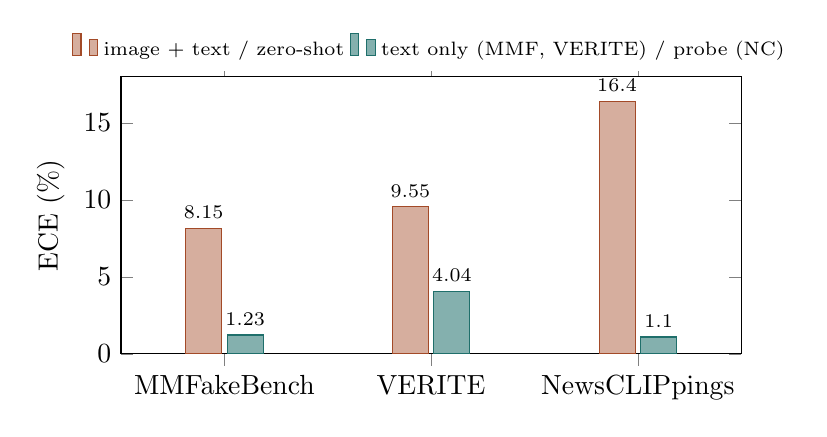
\begin{tikzpicture}
\begin{axis}[
  width=0.78\textwidth,height=5.1cm,ybar,bar width=13pt,ymin=0,ymax=18,
  symbolic x coords={MMFakeBench,VERITE,NewsCLIPpings},xtick=data,
  ylabel={ECE (\%)},enlarge x limits=0.25,
  legend style={draw=none,font=\scriptsize,at={(0.5,1.02)},anchor=south,legend columns=2},
  nodes near coords,nodes near coords style={font=\scriptsize}
]
\addplot[fill=rust!45,draw=rust] coordinates {(MMFakeBench,8.15) (VERITE,9.55) (NewsCLIPpings,16.4)};
\addlegendentry{image + text / zero-shot}
\addplot[fill=teal!55,draw=teal] coordinates {(MMFakeBench,1.23) (VERITE,4.04) (NewsCLIPpings,1.1)};
\addlegendentry{text only (MMF, VERITE) / probe (NC)}
\end{axis}
\end{tikzpicture}
\caption{Calibration error. Text-only is better calibrated than image + text on both datasets; the frozen probe is far better calibrated than zero-shot on NewsCLIPpings. Lower is better.}
\label{fig:ece}
\end{figure}

The source-pair analysis sharpens the first finding. The pooled $-1.51$ pp is an average of large, opposite effects: within-pair differences run from $-18.0$ to $+18.4$ pp; 7 of 14 pairs lie below zero, 2 above, and 5 span zero. The equal-weight mean is $-2.78$ pp, range $[-4.20, -1.47]$. The pooled number describes the source mix in this test split, not a typical per-item image effect.

\begin{figure}[t]
\centering
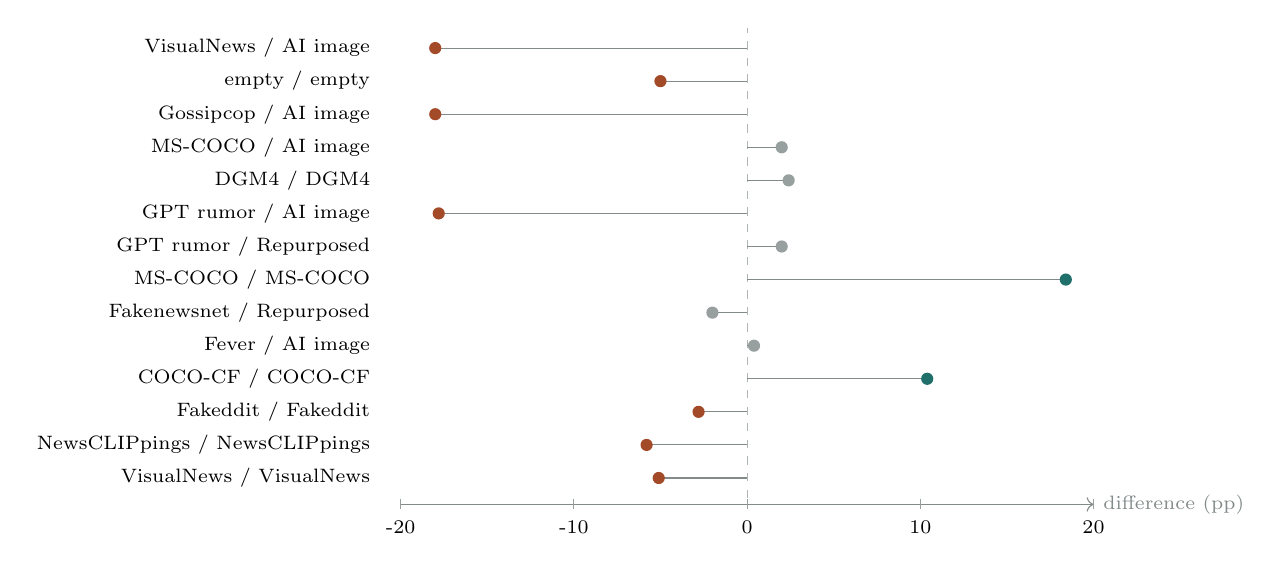
\begin{tikzpicture}[x=0.22cm,y=0.42cm,font=\scriptsize]
\draw[dashed,ink!35] (0,-0.6) -- (0,13.6);
\foreach \v/\c/\lab/\y in {
 -5.1/rust/{VisualNews / VisualNews}/0,
 -5.8/rust/{NewsCLIPpings / NewsCLIPpings}/1,
 -2.8/rust/{Fakeddit / Fakeddit}/2,
 10.4/teal/{COCO-CF / COCO-CF}/3,
 0.4/ink!45/{Fever / AI image}/4,
 -2.0/ink!45/{Fakenewsnet / Repurposed}/5,
 18.4/teal/{MS-COCO / MS-COCO}/6,
 2.0/ink!45/{GPT rumor / Repurposed}/7,
 -17.8/rust/{GPT rumor / AI image}/8,
 2.4/ink!45/{DGM4 / DGM4}/9,
 2.0/ink!45/{MS-COCO / AI image}/10,
 -18.0/rust/{Gossipcop / AI image}/11,
 -5.0/rust/{empty / empty}/12,
 -18.0/rust/{VisualNews / AI image}/13%
} {
  \draw[ink!55] (0,\y) -- (\v,\y);
  \fill[\c] (\v,\y) circle (2.2pt);
  \node[left] at (-21.2,\y) {\lab};
}
\draw[->,ink!55] (-20,-0.8) -- (20,-0.8) node[right]{difference (pp)};
\foreach \x in {-20,-10,0,10,20} { \draw[ink!45] (\x,-0.95) -- (\x,-0.65); \node[below] at (\x,-1.0) {\x}; }
\end{tikzpicture}
\caption{Paired minus text-only accuracy for each of the 14 MMFakeBench source pairs. The pooled effect is $-1.51$ pp, but pairs range from $-18.0$ to $+18.4$ pp: 7 below zero (rust), 2 above (teal), 5 spanning zero (grey). The pooled number describes the source mix, not a typical item.}
\label{fig:pairs}
\end{figure}


NewsCLIPpings is at chance (50.83\%, range $[49.78, 51.81]$), and both probe AUCs are below 0.5 (0.4677 out-of-context, 0.4482 wrong-image). The model over-predicts ``falsified'' (recall 0.90 versus 0.12 for pristine). The frozen probe changes that: on held-out NewsCLIPpings test it reaches 57.4\% versus 51.1\% zero-shot, $+6.24$ pp, range $[4.76, 7.70]$, and calibrates far better (ECE 1.1\% versus 16.4\%). On VERITE true-versus-out-of-context the probe reaches 54.9\% versus 50.5\%, $+4.37$ pp, but the range $[-1.36, 9.95]$ spans zero. The frozen representation carries pairing signal that the zero-shot answer does not use; that is the headroom for fine-tuning.

\subsection{Cross-track synthesis}

\begin{table}[t]
\centering
\small
\caption{What each track contributes. This is a map, not a ranking: datasets, tasks, metrics, and training regimes differ.}
\label{tab:synth}
\begin{tabularx}{\textwidth}{@{}l l l X@{}}
\toprule
\textbf{Track} & \textbf{Regime} & \textbf{Headline} & \textbf{What it establishes} \\
\midrule
Text & Supervised & 87.6--97.4\% acc & Text alone carries strong signal, partly through source and style cues. \\
Image & Supervised & 96.3\% acc, AUC 0.995 & In-distribution detection is strong but brittle under blur. \\
Combined & Zero-shot & 20.37\% macro-F1 & A frozen checkpoint does not use the image; the benchmark is shortcut-solvable. \\
Combined & Frozen probe & 57.4\% NC test & A trained head can recover pairing signal from frozen features. \\
\bottomrule
\end{tabularx}
\end{table}

The comparison that matters is not 96.3\% versus 20.37\%. It is that \emph{supervised} detection on a clean, balanced benchmark can be strong, while a \emph{frozen, zero-shot} model on a fine-grained, shortcut-laden benchmark is weak. The fine-tuning stage exists to test whether a trained head closes that gap, not to make the three numbers look alike.

\section{Discussion and Limits}

\textbf{Benchmark shortcuts.} MMFakeBench labels are largely determined by source names; aggregate accuracy is not a visual-reasoning measure. The same concern applies, in weaker form, to WELFake's ``reuters'' cue. Reporting a shortcut baseline beside every score is mandatory.

\textbf{Exposure and contamination.} The MMFakeBench test split was inspected; the duplicate audit shows non-disjoint content across splits. Pretraining contamination of LAYA-Vision cannot be ruled out, so the zero-shot score is not a clean generalisation estimate.

\textbf{Control validity.} The question bank asks every arm to use ``the supplied image and accompanying text''. The padded arms do not receive both, so the text-only and image-only controls are prompt-mismatched. Paired minus text-only remains directionally conservative because text-only was handicapped, but image-only is not a clean estimate of image-only capability. An arm-specific prompt rerun is the first item of future work.

\textbf{Statistics.} Ranges are descriptive cluster bootstraps, not formal tests; one seed; no multiplicity control. ECE binning differs for NewsCLIPpings. The effective sample for VERITE is 663 images, not 1,001 independent rows.

\textbf{Scope.} One 201M checkpoint, one question bank, one run per arm. Nothing here generalises to other VLMs or to a deployed detector. Text and image results are reported from the track owners' experiments; the combined baseline is verified by 22/22 pipeline gates, an independent 28/28 claims audit, and a deterministic tier-0 check.

\section{Future Work: Fine-Tuning and Setup}

\subsection{Six conditions}

The fine-tuning stage evaluates six conditions on the same rows:
\begin{enumerate}[leftmargin=1.4em,itemsep=1pt]
  \item Zero-shot image + text (the baseline in this paper).
  \item Zero-shot text only (matched control).
  \item Frozen-feature linear probe (this paper; 57.4\% NC test).
  \item Attention head over frozen LAYA features.
  \item Gate head over frozen LAYA features.
  \item CLIP image--text embedding classifier \cite{clip}.
\end{enumerate}
Conditions 1--3 are complete. Conditions 4--6 are the fine-tuning programme.

\subsection{Attention and Gate heads}

Attention and Gate are LAMAR integration methods \cite{lamar}, not LAYA variants; the POS language should be corrected accordingly. We will implement them as fusion heads over the 576-dimensional frozen LAYA decision feature, following the probe protocol. Inputs are image, caption, and their interaction; the head is trained on the 71{,}072 NewsCLIPpings train rows, selected on 7{,}024 validation rows, and scored once on the 7{,}264-row test split and the 663 VERITE true/out-of-context rows. LAYA's weights stay frozen in this stage; end-to-end fine-tuning is a separate, later decision.

\subsection{Targets and decision rule}

The POS targets are 84.8\% on NewsCLIPpings test and 76.3\% on VERITE. Both are \emph{binary true-versus-out-of-context} results from LAMAR, trained end to end. Our VERITE headline (35.66\%) is three-class; the comparable binary number is the probe's 54.9\%. We will report both targets as not met at the baseline, and compare like with like: 57.4\% versus 84.8\% on NewsCLIPpings, and 54.9\% versus 76.3\% on VERITE true-versus-OOC. A head advances only if its gain over the frozen probe has a bootstrap range above zero, or it matches at much lower cost, or it transfers better to unseen generators.

\subsection{Compute and protocol}

The probe ran on Apple MPS in 4.58 hours for 78{,}336 NewsCLIPpings images. Head training is cheap once features are cached; end-to-end fine-tuning needs a GPU (one A100 or equivalent Colab session). The protocol is frozen before any test row is read: fixed splits, fixed prompts, three seeds (13, 29, 47), early stopping on validation, one test read per condition, and paired cluster-bootstrap ranges over exact image bytes. Any model trained on NewsCLIPpings and evaluated on MMFakeBench must first audit image-hash overlap, because 1{,}500 MMFakeBench mismatch rows are sourced from NewsCLIPpings.

\subsection{Captioning and the verdict application}

Two POS items remain separate from the heads: a captioning pipeline (LAYA emits typed decisions, not text) and the Objective~6 Streamlit application that accepts text, image, or both and returns a verdict. The current dashboards are read-only result viewers, not that application. The application will be built over saved predictions first, and only then connected to a model.

\subsection{Ethics and data terms}

All work is non-commercial research. MMFakeBench forbids redistribution of images or derived data; NewsCLIPpings/VisualNews image terms remain unresolved; VERITE images are gated by academic access. We publish aggregate metrics only, store no image corpus for the streamed evaluation, and will not release per-item predictions or images. LAYA-Vision weights are CC BY-NC-SA 4.0; no commercial deployment is planned.

\section{Conclusion}

We presented three coordinated baselines for multimodal misinformation: a supervised text model on WELFake, a supervised image detector on CIFAKE, and a zero-shot combined detector on MMFakeBench, VERITE, and NewsCLIPpings, extended by a frozen-feature probe. The results are useful precisely because they are unflattering: the image adds nothing measurable to the frozen checkpoint, the MMFakeBench benchmark is largely solvable from source metadata, and the CIFAKE detector relies on brittle fine-detail cues. The probe shows that a trained head can recover signal the zero-shot model ignores. The next stage is a pre-registered, six-condition fine-tuning study with three seeds, held-out targets, and an explicit compute and ethics plan.

\appendix
\section{Artifacts and Reproducibility}

Saved predictions and metrics are the source of every number. Combined-track artifacts:
\begin{itemize}[leftmargin=1.2em,itemsep=1pt]
  \item \path{BASELINE_CLAIMS_2026-10-25.md}
  \item \path{BASELINE_REPORT_DRAFT_2026-10-25.md}
  \item \path{controls_metrics_2026-10-25.json}
  \item \path{ncp_metrics_2026-10-25.json}
  \item \path{mmfakebench_test_ablation_2026-10-25.json}
  \item \path{MMFAKEBENCH_SOURCE_PAIR_EFFECT_2026-10-25.md}
  \item \path{FULL_REPORT_ncp_transfer_probe_v1_2026-10-25.md}
\end{itemize}
The main verification command is
\begin{quote}\footnotesize
\texttt{python} \path{data/workflows/analysis/pipeline_status_20261025.py} \texttt{gates}
\end{quote}
which checks coverage arithmetic, gold/manifest agreement, probability sums, accuracy recomputation, and tier-0 determinism (22/22 pass). An independent audit recomputes 28/28 numeric claims with no missing paths. Tier-0: batch 1/4/8 and prefix-cache on produce identical labels and probabilities on the same 300 test rows (maximum delta 0.0). No new inference was used for the paper.

\begin{thebibliography}{99}
\small
\bibitem{welfake} P. K. Verma, P. Agrawal, I. Amorim, and R. Prodan. WELFake: Word embedding over linguistic features for fake news detection. \emph{IEEE Transactions on Computational Social Systems}, 2021.
\bibitem{cifake} J. J. Bird and A. Lotfi. CIFAKE: Image classification and explainable identification of AI-generated synthetic images. \emph{IEEE Access}, 12, 2024.
\bibitem{mmfakebench} MMFakeBench authors. MMFakeBench: A benchmark for multimodal misinformation detection. ICLR, 2025.
\bibitem{verite} S.-I. Papadopoulos et al. VERITE: A robust benchmark for multimodal misinformation detection accounting for unimodal bias. \emph{International Journal of Multimedia Information Retrieval}, 2024.
\bibitem{newsclippings} G. Luo et al. NewsCLIPpings: Automatic generation of out-of-context multimodal media. EMNLP, 2021.
\bibitem{lamar} LAMAR: Multimodal misinformation detection with integration methods. arXiv:2504.06010v3, 2026.
\bibitem{clip} A. Radford et al. Learning transferable visual models from natural language supervision. ICML, 2021.
\bibitem{distilbert} V. Sanh, L. Debut, J. Chaumond, and T. Wolf. DistilBERT, a distilled version of BERT. arXiv:1910.01108, 2019.
\bibitem{resnet} K. He, X. Zhang, S. Ren, and J. Sun. Deep residual learning for image recognition. CVPR, 2016.
\bibitem{smolvlm} Hugging Face. SmolVLM: Small vision-language models. 2025.
\bibitem{laya} N. Kishor et al. LAYA: typed decisions from a small vision-language model. 2025.
\bibitem{wang2020} S.-Y. Wang, O. Wang, R. Zhang, A. Owens, and A. A. Efros. CNN-generated images are surprisingly easy to spot\ldots for now. CVPR, 2020.
\bibitem{frank2020} J. Frank et al. Leveraging frequency analysis for deep fake image recognition. ICML, 2020.
\bibitem{corvi2023} R. Corvi et al. On the detection of synthetic images generated by diffusion models. ICASSP, 2023.
\bibitem{ojha2023} U. Ojha, Y. Li, and Y. J. Lee. Towards universal fake image detectors that generalize across generative models. CVPR, 2023.
\bibitem{genimage} M. Zhu et al. GenImage: A million-scale benchmark for detecting AI-generated images. NeurIPS Datasets and Benchmarks, 2023.
\bibitem{aeroblade} J. Ricker, D. Lukovnikov, and A. Fischer. AEROBLADE: Training-free detection of latent diffusion images using autoencoder reconstruction error. CVPR, 2024.
\bibitem{cozzolino2024} D. Cozzolino et al. Raising the bar of AI-generated image detection with CLIP. CVPR Workshops, 2024.
\bibitem{gradcam} R. R. Selvaraju et al. Grad-CAM: Visual explanations from deep networks via gradient-based localization. ICCV, 2017.
\end{thebibliography}

\end{document}
